\section{Motivation}
Die Motivation dieses Versuchs besteht in der Bestimmung der Planckkonstante mithilfe des Fotoeffekts.
Die Plackkonstante ist eine fundamentale Größe in der Quantenphysik und kennzeichnet die
Quantisierung der Energie. Für die Bestimmung eignet sich der Fotoeffekt,
da dieser eine anschauliche Möglichkeit bietet die Quantisierung des Lichts zu verstehen.


\section{Messverfahren}

Das Licht einer Hg-Dampflampe wird durch einen Kollimator zu einem Doppelprisma geschickt.
Durch den Kollimator sind die Strahlen parallel, weshalb das Licht am Doppelprisma in sein Spektrum zerlegt wird.
Anschließend wird das Licht in einen Kasten gespiegelt. In dem Kasten befindet sich ein Papierschirm,
auf den das Licht mittels eines Hebels umgelenkt werden kann um die gewünschte Spektrallinie zu finden.
Anschließend wird der Hebel umgelegt und mit dem Multimeter das Maximum der messbaren Spannung gesucht.
Dann wird die Vorspannung in $100$ mV Schritten heruntergesetzt und jeweils der Fotostrom mithilfe des Multimeters gemessen.
Der Fotostrom wird mit durch einen Spannungswandler als Spannung abgelesen.
\begin{figure}[h!]
    \centering
    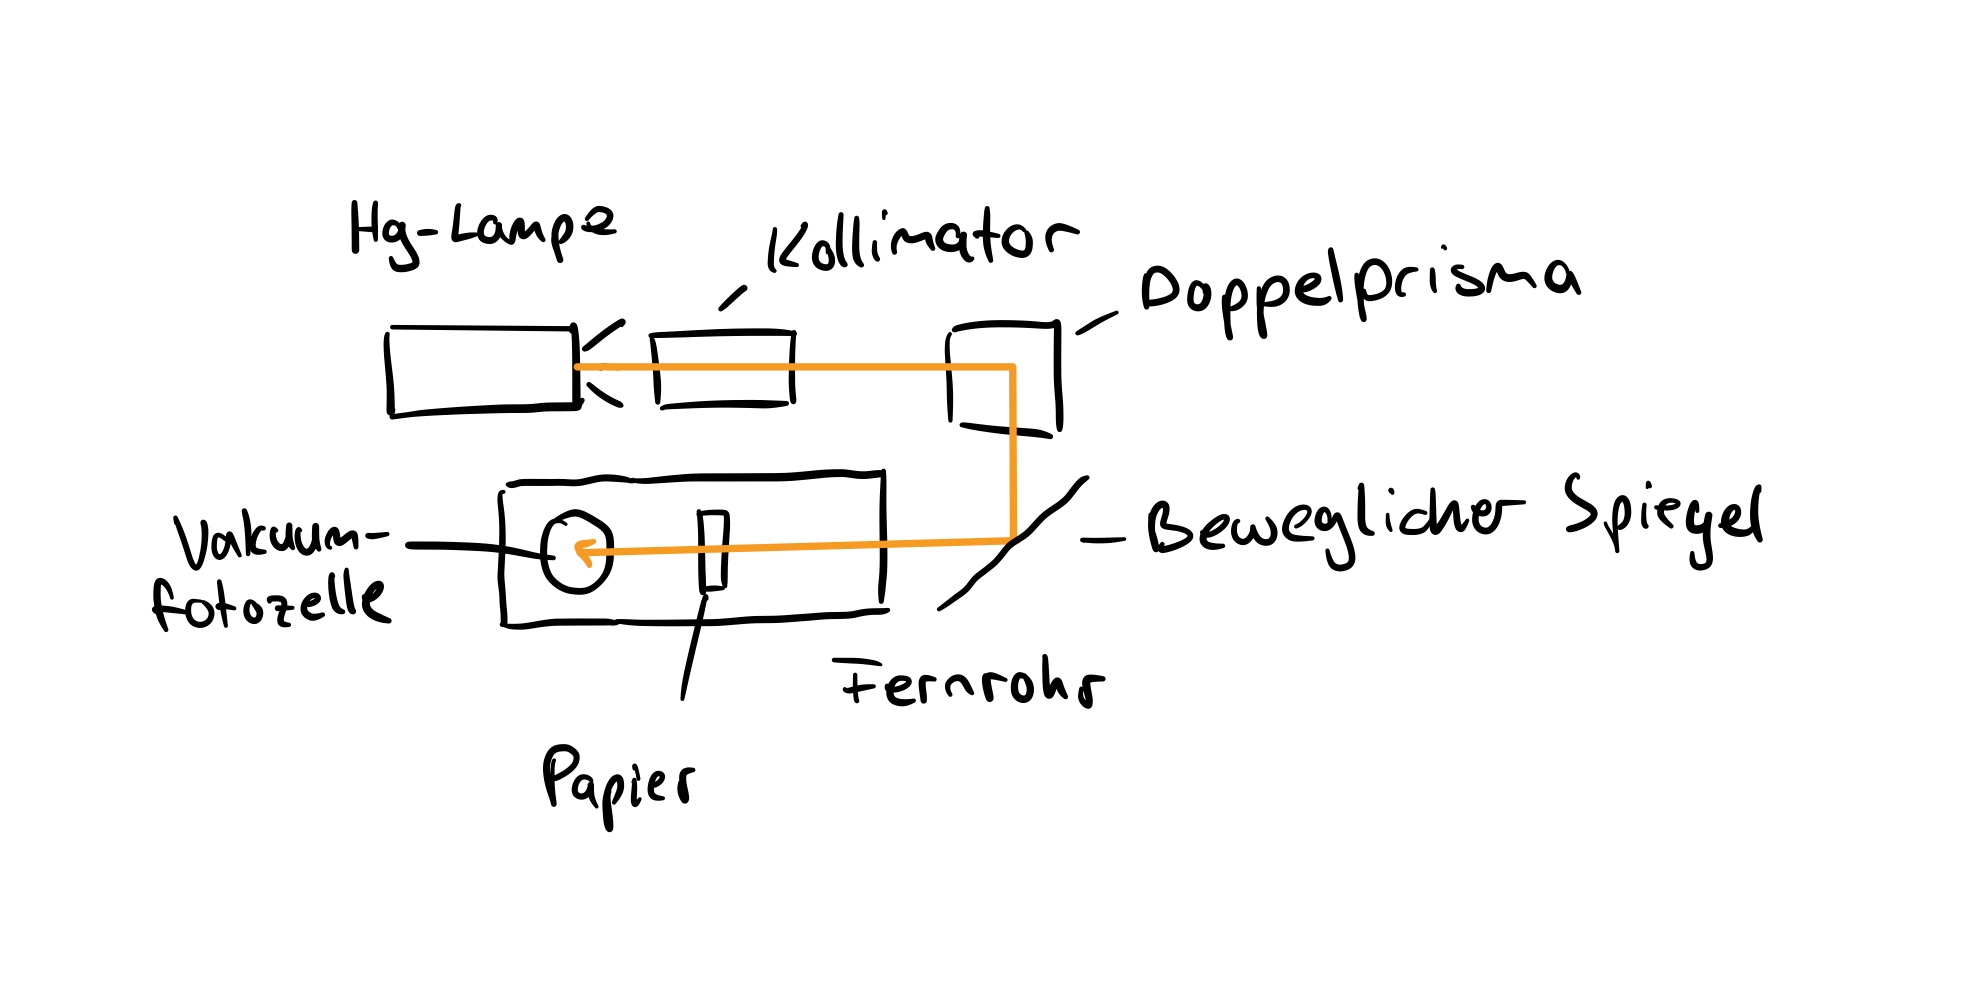
\includegraphics[width=0.9\textwidth,]{35-Skizze.jpeg}
    \caption{Aufbauskizze}
\end{figure}
\section{Grundlagen aus der Physik}
\subsection{Fotozelle}

Die Photozelle besteht aus einer Kathode, aus welcher mithilfe von Licht Elektronen ausgelöst werden können.


\begin{equation}
    I \propto U_I - U_{I0}
\end{equation}
\begin{equation}
    U \propto \sqrt{I} 
\end{equation}
\begin{equation}
    U \propto \sqrt{U_I - U_{I0}} 
\end{equation}

\section{Standartabweichung}
Allgemein lässt sich die Abweichung eines Messwertes $x$ zu einem Literaturwert $x_{Lit}$ darstellen durch die Sigmaabweichung:

\begin{equation}
    \frac{|x-x_{Lit}|}{\Delta x} = k \sigma \ \ mit \ k \in \mathbb{R}
    \label{eq:sigma}
\end{equation}
